\documentclass[presentation,xcolor={table},9pt]{beamer}

\usepackage{adjustbox}
\usepackage{algorithm}
\usepackage{algpseudocode}
\usepackage{amsfonts}
\usepackage{amsmath}
\usepackage{amssymb}
\usepackage{amsthm}
\usepackage{bookmark}
\usepackage{booktabs}
\usepackage[makeroom]{cancel}
\usepackage[american]{circuitikz}
\usepackage{cite}
% \usepackage{fixmath}
\usepackage[acronym]{glossaries-extra}
\usepackage{hyperref}
\usepackage{import}
\usepackage{mathtools}
\usepackage{microtype}
\usepackage[short]{optidef}
\usepackage{pgfplots}
\usepackage{ragged2e}
\usepackage{siunitx}
\usepackage{stfloats}
\usepackage[caption=false,font=footnotesize,subrefformat=parens,labelformat=parens]{subfig}
\usepackage{tabularx}
\usepackage{tikz}
\usepackage{graphicx}
\usepackage{epstopdf}
\usepackage{multirow}
\usepackage{booktabs}
\usepackage{lastpage}
\usepackage{caption}
\setbeamerfont{caption}{size=\footnotesize}
\captionsetup[figure]{labelformat=empty}
\usefonttheme[onlymath]{serif}

\makeatletter
\@addtoreset{subfigure}{framenumber}
\makeatother

\makeatletter
\newcommand{\forcealgorithm}{\let\@latex@error\@gobble}
\makeatother

% footnote
\newcommand\blfootnote[1]{%
\begingroup
\renewcommand\thefootnote{}\footnote{#1}%
\addtocounter{footnote}{-1}%
\endgroup
}

% amsthm
\newtheorem{proposition}{Proposition}
\newtheorem{remark}{Remark}
% \newtheorem{lemma}{Lemma}
% \newtheorem{corollary}{Corollary}[proposition]

% PGF/TikZ
\pgfplotsset{compat=1.18}
\usepgfplotslibrary{fillbetween,groupplots,patchplots}
\usetikzlibrary{arrows,arrows.meta,automata,backgrounds,calc,math,matrix,patterns,plotmarks,positioning,shapes,angles,quotes}
\usetikzlibrary{decorations.pathmorphing,decorations.pathreplacing,decorations.markings,decorations.shapes,shapes.geometric}

% glossaries-extra
\glsdisablehyper
\setabbreviationstyle[acronym]{long-short}
\newacronym{ai}{AI}{Artificial Intelligence}
\newacronym{af}{AF}{Amplify-and-Forward}
\newacronym{ambc}{AmBC}{Ambient Backscatter Communication}
\newacronym{am}{AM}{Arithmetic Mean}
\newacronym{ao}{AO}{Alternating Optimization}
\newacronym{ap}{AP}{Access Point}
\newacronym{apm}{APM}{Amplitude-Phase Modulation}
\newacronym{awgn}{AWGN}{Additive White Gaussian Noise}
\newacronym{bbc}{BBC}{Bistatic Backscatter Communication}
\newacronym{bcd}{BCD}{Block Coordinate Descent}
\newacronym{bc}{BackCom}{Backscatter Communication}
\newacronym{bd}{BD}{Beyond-Diagonal}
\newacronym{ber}{BER}{Bit Error Rate}
\newacronym{bibo}{BIBO}{Binary-Input Binary-Output}
\newacronym{bls}{BLS}{Backtracking Line Search}
\newacronym{bpcu}{\si{bpcu}}{bits per channel use}
\newacronym{bpsphz}{\si{bps/Hz}}{bits per second per Hertz}
\newacronym{clt}{CLT}{Central Limit Theorem}
\newacronym{cp}{CP}{Canonical Polyadic}
\newacronym{cr}{CR}{Cognitive Radio}
\newacronym{cscg}{CSCG}{Circularly Symmetric Complex Gaussian}
\newacronym{csit}{CSIT}{Channel State Information at the Transmitter}
\newacronym{csi}{CSI}{Channel State Information}
\newacronym{cw}{CW}{Continuous Waveform}
\newacronym{d2d}{D2D}{Device-to-Device}
\newacronym{dcmc}{DCMC}{Discrete-input Continuous-output Memoryless Channel}
\newacronym{dc}{DC}{Direct Current}
\newacronym{df}{DF}{Decode-and-Forward}
\newacronym{dmc}{DMC}{Discrete Memoryless Channel}
\newacronym{dmmac}{DMMAC}{Discrete Memoryless Multiple Access Channel}
\newacronym{dmtc}{DMTC}{Discrete Memoryless Thresholding Channel}
\newacronym{dof}{DoF}{Degree of Freedom}
\newacronym{dp}{DP}{Dynamic Programming}
\newacronym{eirp}{EIRP}{Effective Isotropic Radiated Power}
\newacronym{fdma}{FDMA}{Frequency-Division Multiple Access}
\newacronym{fpga}{FPGA}{Field-Programmable Gate Array}
\newacronym{gm}{GM}{Geomtric Mean}
\newacronym{gp}{GP}{Geometric Programming}
\newacronym{ic}{IC}{Interference Channel}
\newacronym{iid}{i.i.d.}{independent and identically distributed}
\newacronym{im}{IM}{Index Modulation}
\newacronym{ioe}{IoE}{Internet of Everything}
\newacronym{iot}{IoT}{Internet of Things}
\newacronym{kkt}{KKT}{Karush-Kuhn-Tucker}
\newacronym{los}{LoS}{Line-of-Sight}
\newacronym{m2m}{M2M}{Machine-to-Machine}
\newacronym{mac}{MAC}{Multiple Access Channel}
\newacronym{mbc}{MBC}{Monostatic Backscatter Communication}
\newacronym{mc}{MC}{Multiplication Coding}
\newacronym{mimo}{MIMO}{Multiple-Input Multiple-Output}
\newacronym{miso}{MISO}{Multiple-Input Single-Output}
\newacronym{ml}{ML}{Maximum-Likelihood}
\newacronym{mmse}{MMSE}{Minimum Mean-Square-Error}
\newacronym{mrc}{MRC}{Maximal Ratio Combining}
\newacronym{mrt}{MRT}{Maximum Ratio Transmission}
\newacronym{mse}{MSE}{Mean-Square Error}
\newacronym{nlos}{NLoS}{Non-Line-of-Sight}
\newacronym{noma}{NOMA}{Non-Orthogonal Multiple Access}
\newacronym{ofdm}{OFDM}{Orthogonal Frequency-Division Multiplexing}
\newacronym{pc}{PC}{Point-to-point Channel}
\newacronym{pdf}{PDF}{Probability Density Function}
\newacronym{pga}{PGA}{Projected Gradient Ascent}
\newacronym{pin}{PIN}{Positive Intrinsic Negative}
\newacronym{psk}{PSK}{Phase Shift Keying}
\newacronym{ps}{PS}{Power Splitting}
\newacronym{qam}{QAM}{Quadrature Amplitude Modulation}
\newacronym{qos}{QoS}{Quality of Service}
\newacronym{r-e}{R-E}{Rate-Energy}
\newacronym{rcg}{RCG}{Riemannian Conjugate Gradient}
\newacronym{rfid}{RFID}{Radio-Frequency Identification}
\newacronym{rf}{RF}{Radio-Frequency}
\newacronym{ris}{RIS}{Reconfigurable Intelligent Surface}
\newacronym{sca}{SCA}{Successive Convex Approximation}
\newacronym{sc}{SC}{Superposition Coding}
\newacronym{sdma}{SDMA}{Space-Division Multiple Access}
\newacronym{sdp}{SDP}{Semi-Definite Programming}
\newacronym{sdr}{SDR}{Semi-Definite Relaxation}
\newacronym{sic}{SIC}{Successive Interference Cancellation}
\newacronym{simo}{SIMO}{Single-Input Multiple-Output}
\newacronym{sinr}{SINR}{Signal-to-Interference-plus-Noise Ratio}
\newacronym{siso}{SISO}{Single-Input Single-Output}
\newacronym{smawk}{SMAWK}{Shor-Moran-Aggarwal-Wilber-Klawe}
\newacronym{star}{STAR}{Simultaneous Transmission and Reflection}
\newacronym{smf}{SMF}{Scaled Matched Filter}
\newacronym{snr}{SNR}{Signal-to-Noise Ratio}
\newacronym{sr}{SR}{Symbiotic Radio}
\newacronym{svd}{SVD}{Singular Value Decomposition}
\newacronym{swipt}{SWIPT}{Simultaneous Wireless Information and Power Transfer}
\newacronym{tdma}{TDMA}{Time-Division Multiple Access}
\newacronym{ts}{TS}{Time Switching}
\newacronym{ue}{UE}{User Equipment}
\newacronym{wf}{WF}{Water-Filling}
\newacronym{wit}{WIT}{Wireless Information Transfer}
\newacronym{wpcn}{WPCN}{Wireless Powered Communication Network}
\newacronym{wpt}{WPT}{Wireless Power Transfer}
\newacronym{wsn}{WSN}{Wireless Sensor Network}
\newacronym{wsr}{WSR}{Weighted Sum-Rate}
\newacronym{zf}{ZF}{Zero-Forcing}
\newacronym{lc}{LC}{Low-Complexity}
\newacronym{ble}{BLE}{Bluetooth Low Energy}
\newacronym{lora}{LoRa}{Long Range}
\newacronym{lorawan}{LoRaWAN}{Long Range Wide Area Network}
\newacronym{pae}{PAE}{Power-Added Efficiency}
\newacronym{papr}{PAPR}{Peak-to-Average Power Ratio}
\newacronym{fsk}{FSK}{Frequency-Shift Keying}
\newacronym{css}{CSS}{Chirp Spread Spectrum}
\newacronym{dsss}{DSSS}{Direct-Sequence Spread Spectrum}
\newacronym{fsss}{FSSS}{Frequency-Hopping Spread Spectrum}
\newacronym{rz}{RZ}{Return-to-Zero}
\newacronym{nrz}{NRZ}{Non-Return-to-Zero}
\newacronym{leh}{LEH}{Linear Energy Harvester}
\newacronym{fs}{FS}{Frequency-Selective}
\newacronym{rsma}{RSMA}{Rate-Splitting Multiple Access}

\newacronym{embb}{eMBB}{enhanced Mobile Broadband}
\newacronym{urllc}{URLLC}{Ultra-Reliable Low-Latency Communication}
\newacronym{mmtc}{mMTC}{massive Machine-Type Communication}


\usetheme{Frankfurt}
\addtobeamertemplate{navigation symbols}{}{%
    \usebeamerfont{footline}%
    \usebeamercolor[fg]{footline}%
    \hspace{1em}%
	\raisebox{1.5pt}[0pt][0pt]{\insertframenumber/\inserttotalframenumber}
}

\epstopdfsetup{outdir=../assets/viva/}

\title[\glsfmtshort{ris}: Beamforming, Modulation, and Channel Shaping]{\textbf{\glsfmtfull{ris}:\\Beamforming, Modulation, and Channel Shaping}}
\subtitle{Viva Presentation}
\author{Yang Zhao, supervised by Prof Bruno Clerckx}
\institute{Department of Electrical and Electronic Engineering\\Imperial College London}
% \date{\today}
\date{May 2, 2024}

\begin{document}

\frame{\titlepage}


\begin{section}{Intro}
	\begin{frame}{Do we want more waves in the air?}
		\begin{block}{Massive \glsfmtshort{mimo} is here}
			\begin{figure}
				\centering
				\subfloat[8T8R and m\glsfmtshort{mimo} at Imperial]{
					\resizebox{!}{3cm}{
						\includegraphics{../assets/viva/massive_mimo.jpg}
					}
				}
				\subfloat[Cellular statistics]{
					\resizebox{!}{3cm}{
						\includegraphics{../assets/viva/cellular_analysis.png}
					}
				}
			\end{figure}
		\end{block}
		\begin{block}{How far are we from the Shannon capacity?}
			\begin{equation*}
				C(\mathbf{H}) = \max_{\mathbf{Q} \succeq 0, \mathrm{tr}(\mathbf{Q}) \le P} \log \det \left( \mathbf{I} + \rho \mathbf{H} \mathbf{Q} \mathbf{H}^\mathsf{H} \right)
			\end{equation*}
			\vspace{-1em}
			\begin{itemize}
				\item Modulation, coding, and beamforming to \textcolor{gray}{adapt to} the stochastic channel
				\item \gls{ris} can \textcolor{blue}{shape and control} the channel
			\end{itemize}
		\end{block}
	\end{frame}

	\begin{frame}{What is \glsfmtshort{ris}?}
		A planar surface of controllable scattering elements for signal amplitude and phase manipulation \cite{Wu2020}.
		\begin{figure}
			\centering
			\includegraphics[width=0.65\textwidth]{../assets/viva/ris_architecture.pdf}
			\label{fg:ris_architecture}
		\end{figure}
		\begin{block}{Characteristics}
			\begin{itemize}
				\item Low-power and low-cost
				\item Negligible noise and latency
				\item Full-duplex without self-interference
				\item Programmable in real-time
			\end{itemize}
		\end{block}
	\end{frame}

	\begin{frame}{Use cases of \glsfmtshort{ris}}
		\begin{itemize}
			\item \textcolor{blue}{Beamforming} of \gls{ris} and transceiver can be jointly designed for a specific performance measure.
			\item \gls{ris} can be used for backscatter \textcolor{blue}{modulation} by periodically switching the reflection pattern.
			\item \textcolor{blue}{Channel shaping} exploits the \gls{ris} as a stand-alone device to modify the inherent properties of the propagation environment.
		\end{itemize}

		\begin{figure}
			\centering
			\subfloat[Beamforming \cite{Wu2020}]{
				\resizebox{0.32\textwidth}{!}{
					\includegraphics{../assets/viva/ris_beamforming_swipt.jpg}
				}
			}
			\subfloat[Modulation \cite{Hu2021a}]{
				\resizebox{0.32\textwidth}{!}{
					\includegraphics{../assets/viva/ris_modulation.pdf}
				}
			}
			\subfloat[Channel shaping \cite{Arslan2022}]{
				\resizebox{0.32\textwidth}{!}{
					\includegraphics{../assets/viva/ris_shaping.pdf}
				}
			}
		\end{figure}
	\end{frame}
\end{section}

\begin{section}{Beamforming: \glsfmtshort{ris}-Aided \glsfmtshort{swipt}}
	\begin{frame}{\glsfmtshort{ris}-aided \glsfmtshort{swipt}: Joint waveform and beamforming design}
		\begin{block}{Overview}
			\begin{itemize}\setlength\itemsep{20pt}
				\item \textit{What does this paper propose?}

				A single-user multi-carrier \gls{swipt} system aided by a passive \gls{ris}.
				\item \textit{How does it differ from previous work?}

				We consider waveform and beamforming design for practical receiver architectures under non-linear harvester and frequency-flat \gls{ris} models.
				\item \textit{What are the benefits?}

				It exploits the spatial-frequency domain and rectifier behavior to enlarge the \gls{r-e} region, achieving squared asymptotic performance than conventional designs.
			\end{itemize}
		\end{block}
	\end{frame}

	\begin{frame}{From received signal to harvested power}
		The rectenna efficiency $\eta_3$ depends on its input waveform (power and shape).
		\begin{block}{Rectenna model}
			\begin{itemize}
				\item Linear region (constant $\eta_3$): $P_{\mathrm{DC}}^\mathrm{R} = \eta_3 P_\mathrm{RF}^\mathrm{R} = \eta_3 \mathbb{A}\bigl\{ \lvert y(t) \rvert^2 \bigr\}$
				\item Non-linear region: Taylor expansion on diode characteristic equation
				\vspace{-0.25cm}
				\begin{equation*}
					\arg_{x(t)} \max P_{\mathrm{DC}}^\mathrm{R} = \arg_{x(t)} \max z \triangleq \sum_{i=2,\text{even}}^{n_0} \beta_i \mathbb{A}\bigl\{ y^i(t) \bigr\},
					\vspace{-0.5cm}
				\end{equation*}
				where $\beta_i = I_\mathrm{S} \frac{R_\mathrm{A}^{i/2}}{i!(n v_\mathrm{T})^i}$ is a constant and $n_0$ is the truncation order.
			\end{itemize}
		\end{block}
		\begin{alertblock}{In multi-carrier \glsfmtshort{wpt} \textellipsis}
			\begin{itemize}
				\item $n_0 \ge 4$ allows components to compensate each other for higher \glsfmtshort{dc} power
				\item High \gls{papr} (e.g., multi-sine) is preferred \cite{Trotter2009}
			\end{itemize}
			\vspace{-0.5cm}
			\begin{figure}
				\centering
				\subfloat{
					\resizebox{!}{2.5cm}{
						\includegraphics{../assets/viva/multisine_frequency_domain.eps}
					}
				}
				\subfloat{
					\resizebox{!}{2.5cm}{
						\includegraphics{../assets/viva/multisine_time_domain.eps}
					}
				}
			\end{figure}
		\end{alertblock}
	\end{frame}

	\begin{frame}{From \glsfmtshort{wpt} to \gls{ris}-aided \glsfmtshort{swipt}}
		\begin{figure}[H]
			\centering
			\def\svgwidth{0.3\columnwidth}
			\input{../assets/viva/system.eps_tex}
		\end{figure}

		\begin{itemize}
			\item \gls{swipt} features shared signal, spectrum, and infrastructure
			\item \gls{ris} enhances the RF-to-RF efficiency $\eta_2$ which has been a major concern
		\end{itemize}
		\begin{block}{Transmit waveform}
			\begin{equation*}
				\mathbf{x}(t) = \Re \left\{\sum_{n=1}^N \Bigl(\mathbf{w}_{\mathrm{I},n} \cdot \underbrace{\tilde{x}_{\mathrm{I},n}(t) e^{\jmath 2{\pi}{f_n}{t}}}_\text{modulated}+\mathbf{w}_{\mathrm{P},n} \cdot \underbrace{e^{\jmath 2{\pi}{f_n}{t}}}_\text{multi-sine}\Bigr) \right\}
			\end{equation*}
		\end{block}
		\begin{block}{Receiver architectures}
			\vspace{-0.5cm}
			\begin{figure}
				\centering
				\subfloat[\gls{ts} receiver]{
					\resizebox{0.35\columnwidth}{!}{
						\begin{circuitikz}[transform shape,align=center]
	\draw (0,0) node[bareRXantenna](r){Rx}(r.center)
		to[short] ++(0,-1) node[below]{Time switcher}
		to[short] node[spdt,anchor=in](s){} ++(0.5,0);

	\draw (s.out 1)
		to ++(1.25,0)
		to ++(0,0.5)
		to ++(1,0) node[draw,minimum width=2.5cm,anchor=west](eh){Energy\\harvester};
	% \draw (eh.east) to ++(1,0) node[draw,anchor=west,minimum width=2.5cm]{Power\\management};

	\draw (s.out 2)
		to ++(1.25,0)
		to ++(0,-0.5)
		to ++(1,0) node[draw,anchor=west,minimum width=2.5cm]{Information\\decoder};
\end{circuitikz}

% \begin{circuitikz}[transform shape,align=center]
% 	\draw (0,0) node[bareRXantenna](r){Rx}(r.center)
% 		to[short] ++(0,-1)
% 		to node[coupler,anchor=left up](c){Power splitter} ++(1,0);
% 	\draw (c.right up)
% 		to[short] ++(0.5,0)
% 		to ++(0,0.5)
% 		to ++(1,0) node[draw,minimum width=2.5cm,anchor=west](eh){Energy\\harvester};
% 	\draw (eh.east) to ++(1,0) node[draw,anchor=west,minimum width=2.5cm]{Power\\management};
% 	\draw (c.right down)
% 		to[short] ++(0.5,0)
% 		to ++(0,-0.5)
% 		to ++(1,0) node[draw,anchor=west,minimum width=2.5cm]{Information\\decoder};
% \end{circuitikz}

					}
					\label{fg:receiver_ts}
				}
				\subfloat[\gls{ps} receiver]{
					\resizebox{0.35\columnwidth}{!}{
						\begin{circuitikz}[transform shape,align=center]
	\draw (0,0) node[bareRXantenna](r){Rx}(r.center)
		to[short] ++(0,-1)
		to node[coupler,anchor=left up](c){Power splitter} ++(1,0);
	\draw (c.right up)
		to[short] ++(0.5,0)
		to ++(0,0.5)
		to ++(1,0) node[draw,minimum width=2.5cm,anchor=west](eh){Energy\\harvester};
	% \draw (eh.east) to ++(1,0) node[draw,anchor=west,minimum width=2.5cm]{Power\\management};
	\draw (c.right down)
		to[short] ++(0.5,0)
		to ++(0,-0.5)
		to ++(1,0) node[draw,anchor=west,minimum width=2.5cm]{Information\\decoder};
\end{circuitikz}

					}
					\label{fg:receiver_ps}
				}
			\end{figure}
		\end{block}
	\end{frame}

	\begin{frame}{Joint waveform and beamforming design}
		\begin{block}{Problem formulation}
			\vspace{-0.25cm}
			\begin{maxi*}
				{\scriptstyle{\boldsymbol{\theta},\mathbf{W}_\mathrm{I},\mathbf{W}_\mathrm{P},\rho}}{z(\boldsymbol{\theta},\mathbf{W}_\mathrm{I},\mathbf{W}_\mathrm{P},\rho)}{}{}
				\addConstraint{\lVert{\mathbf{W}_{\mathrm{I}}}\rVert _\mathrm{F}^2/2 + \lVert{\mathbf{W}_{\mathrm{P}}}\rVert _\mathrm{F}^2/2\le{P}}
				\addConstraint{R(\boldsymbol{\theta},\mathbf{W}_\mathrm{I},\rho) \ge \bar{R}}
				\addConstraint{\lvert{\phi_l}\rvert=1, \quad l=1,\dots,L}
				\addConstraint{0 \le \rho \le 1,}
			\end{maxi*}
		\end{block}
		\begin{exampleblock}{Solution by \glsfmtfull{bcd}}
			\begin{itemize}
				\item Optimally decouple the spatial and frequency domain design
				\begin{equation*}
					\mathbf{w}_{\mathrm{I/P}, n} = \underbrace{s_{\mathrm{I/P}, n}}_\text{frequency} \underbrace{\mathbf{p}_{\mathrm{I/P}, n}}_\text{spatial}
				\end{equation*}
				\item Active beamforming $\mathbf{p}$: \gls{mrt}
				\item Passive beamforming $\boldsymbol{\theta}$: \gls{sca}
				\item Power allocation $\mathbf{s}$ and splitting ratio $\rho$: \gls{gp}
			\end{itemize}
		\end{exampleblock}
	\end{frame}

	\begin{frame}{Simulation results: Asymptotic behavior}
		\begin{figure}
			\centering
			\subfloat[Number of transmit antennas $M$]{
				\resizebox{0.45\columnwidth}{!}{
					\input{../assets/viva/scaling_tx.tex}
				}
			}
			\subfloat[Number of \gls{ris} elements $L$]{
				\resizebox{0.45\columnwidth}{!}{
					\input{../assets/viva/scaling_reflector.tex}
				}
			}
		\end{figure}
		\begin{itemize}
			\item Active beamforming: array gain $M$ and harvested power order $M^2$
			\item Passive beamforming: array gain $L^2$ and harvested power order $L^4$
			\item Superlinear thanks to coherent scattering and rectifier nonlinearity
		\end{itemize}
	\end{frame}
\end{section}

\begin{section}{Modulation: RIScatter}
	\begin{frame}{RIScatter: Unifying \gls{bc} and \glsfmtshort{ris}}
		\begin{block}{Overview}
			\begin{itemize}\setlength\itemsep{20pt}
				\item \textit{What does this paper propose?}

				RIScatter --- a batteryless cognitive radio that recycles ambient signal in an adaptive and customizable manner.
				\item \textit{How does it differ from previous work?}

				Backscatter modulation and passive beamforming are seamlessly integrated from the perspective of probability distribution.
				\item \textit{What are the benefits?}

				It supports cooperative and distributed deployment, avoids complex architecture and signal processing, and can be built over legacy systems.
			\end{itemize}
		\end{block}
	\end{frame}

	\begin{frame}{Signal model}
		RIScatter renders the node input distribution as a function of information source, \gls{csi}, and priority of coexisting links.
		\begin{figure}[H]
			\centering
			\def\svgwidth{0.6\columnwidth}
			\input{../assets/viva/riscatter_network.pdf_tex}
			\label{fg:riscatter_network}
		\end{figure}
		\begin{equation*}
			y[n] = \underbrace{\Bigl(\mathbf{h}_{\text{D}}^\mathsf{H} + \sum_{k} \alpha_k \mathbf{h}_{\text{C},k}^\mathsf{H} \textcolor{orange}{x_k}\Bigr)}_{\mathbf{h}^\mathsf{H}(\textcolor{orange}{x_{\mathcal{K}}})} \mathbf{w} \textcolor{blue}{s[n]} + v[n],
		\end{equation*}
		\vspace{-0.25cm}
		\begin{block}{Properties}
			\begin{enumerate}
				\item \textcolor{blue}{Primary} and \textcolor{orange}{backscatter} symbols are superimposed by {double modulation}
				\item Backscatter signal is much weaker due to {double fading}
				\item The spreading factor (i.e., symbol period ratio $N$) is usually large
				\item Each {state} is simultaneously part of information and beamforming {codeword}
				\item Reflection pattern over time is guided by input probability distribution
			\end{enumerate}
		\end{block}
	\end{frame}

	\begin{frame}{Low-complexity receiver}
		We propose a low-complexity receiver that exploits the aforementioned properties to avoid \gls{sic}.
		\begin{figure}[!t]
			\centering
			\subfloat{
				\resizebox{0.42\linewidth}{!}{
					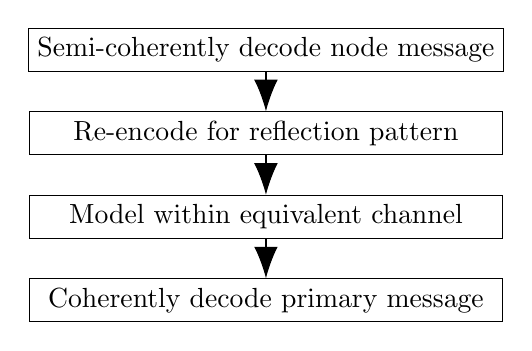
\begin{tikzpicture}[
		% every axis plot/.append style={thick},
		every node/.append style={draw,minimum width=6cm},
		align=center
	]
	\draw[-{Latex[length=4mm]}] (0,0) node[anchor=south](0){Semi-coherently decode node message} to ++(0,-0.5) node[anchor=north](1){Re-encode for reflection pattern};
	\draw[-{Latex[length=4mm]}] (1.south) to ++(0,-0.5) node[anchor=north](2){Model within equivalent channel};
	\draw[-{Latex[length=4mm]}] (2.south) to ++(0,-0.5) node[anchor=north](3){Coherently decode primary message};
\end{tikzpicture}

				}
			}
			\subfloat{
				\resizebox{0.58\linewidth}{!}{
					\input{../assets/viva/energy_distribution.tex}
				}
			}
			\label{fg:receiver}
		\end{figure}
		\vspace{0.5cm}
		\begin{itemize}
			\item Accumulated receive energy $z=\sum_{n} \bigl\lvert y[n] \bigr\rvert^2$ follows Gamma distribution
			\item \textcolor{orange}{Backscatter detection} under primary uncertainty is part of \textcolor{blue}{channel training}
			\item Requires one energy comparison and re-encoding per backscatter symbol (much simpler than symbiotic radio with $N$ \gls{sic} and 1 combining)
		\end{itemize}
	\end{frame}

	\begin{frame}{Joint beamforming, input distribution, and energy detector design}
		\begin{block}{Problem formulation}
			\vspace{-0.25cm}
			\begin{maxi*}
				{\scriptstyle{\{\mathbf{p}_k\},\mathbf{w},\mathbf{t}}}{\rho R_\text{P} + (1-\rho) \sum\nolimits_{k} R_{\text{B},k}}{}{}
				\addConstraint{\mathbf{1}^\mathsf{T} \mathbf{p}_k=1,}{\quad \mathbf{p}_k \ge \mathbf{0},}{\quad \forall k}
				\addConstraint{t_{l-1} \le t_l,}{\quad t_l \ge 0,}{\quad \forall l}
				\addConstraint{\lVert \mathbf{w} \rVert^2 \le P,}{}{}
			\end{maxi*}
		\end{block}
		\begin{exampleblock}{Solution by \gls{bcd}}
			\begin{itemize}
				\item Input distribution $\{\mathbf{p}_k\}$: \gls{kkt}
				\item Active beamforming $\mathbf{w}$: \gls{pga}
				\item Energy decision threshold $\mathbf{t}$: \gls{dp}
			\end{itemize}
		\end{exampleblock}
	\end{frame}

	\begin{frame}{Simulation results: Input distribution and rate region}
		\begin{figure}[!t]
			\centering
			\subfloat{
				\resizebox{0.48\linewidth}{!}{
					\input{../assets/viva/distribution_weights.tex}
				}
			}
			\subfloat{
				\resizebox{0.48\linewidth}{!}{
					\input{../assets/viva/region_comparison.tex}
				}
			}
		\end{figure}
		\begin{itemize}
			\item Increasing $\rho$ from 0 to 1 evolves from \gls{bc} to \gls{ris}
			\item Backscatter rate is lower than \glsfmtshort{sr} (due to energy detection) but higher than \glsfmtshort{ambc} (due to adaptive encoding)
			\item Active and passive transmission can share resource with mutual benefits
			% creates a smooth transition from backscatter modulation to passive beamforming
		\end{itemize}
	\end{frame}
\end{section}

\begin{section}{Shaping: \glsfmtshort{bd}-\glsfmtshort{ris} in \glsfmtshort{mimo}}
	\begin{frame}{Channel shaping using \glsfmtshort{ris}: From diagonal model to beyond}
		\begin{block}{Overview}
			\begin{itemize}\setlength\itemsep{20pt}
				\item \textit{What does this paper study?}

				To what extent can a passive \gls{ris} redistribute the singular values of a \gls{mimo} channel.
				\item \textit{How does it differ from previous work?}

				We consider a \gls{bd} architecture, depict the singular value region, derive analytical bounds, and solve the rate maximization problem.
				\item \textit{What are the benefits?}

				Channel shaping is ubiquitous for communication, sensing, and power transfer, which helps to decouple the \gls{ris}-transceiver design.
				We also propose an efficient and universal \gls{bd}-\gls{ris} design framework.
			\end{itemize}
		\end{block}
	\end{frame}

	\begin{frame}{Wave scattering model}
		\begin{block}{Diagonal \glsfmtshort{ris}}
			Each element acts as an individual scatterer with phase shift only
			\begin{equation*}
				\mathbf{\Theta} = \mathrm{diag}(\theta_1, \ldots, \theta_{N_\mathrm{S}}) = \mathrm{diag}(e^{\jmath \phi_1}, \ldots, e^{\jmath \phi_{N_\mathrm{S}}})
				%  =
				% \begin{bsmallmatrix}
				% 	\theta_1 & 0 & \cdots & 0 \\
				% 	0 & \theta_2 & \cdots & 0 \\
				% 	\vdots & \vdots & \ddots & \vdots \\
				% 	0 & 0 & \cdots & \theta_{N_\mathrm{S}}
				% \end{bsmallmatrix}
				\label{eq:diagonal_scattering_matrix}
			\end{equation*}
		\end{block}

		\begin{block}{\glsfmtshort{bd}-\glsfmtshort{ris}}
			Each group contains $L$ connected elements, allowing amplitude and phase control
			% \vspace{-0.25cm}
			\begin{equation*}
				\mathbf{\Theta} = \mathrm{diag}(\mathbf{\Theta}_1,\ldots,\mathbf{\Theta}_G), \quad \mathbf{\Theta}_g^\mathsf{H} \mathbf{\Theta}_g = \mathbf{I}_L, \quad \forall g
				\label{eq:bd_ris}
			\end{equation*}
			\vspace{-0.5cm}
			\begin{figure}[H]
				\centering
				\resizebox{0.5\columnwidth}{!}{
					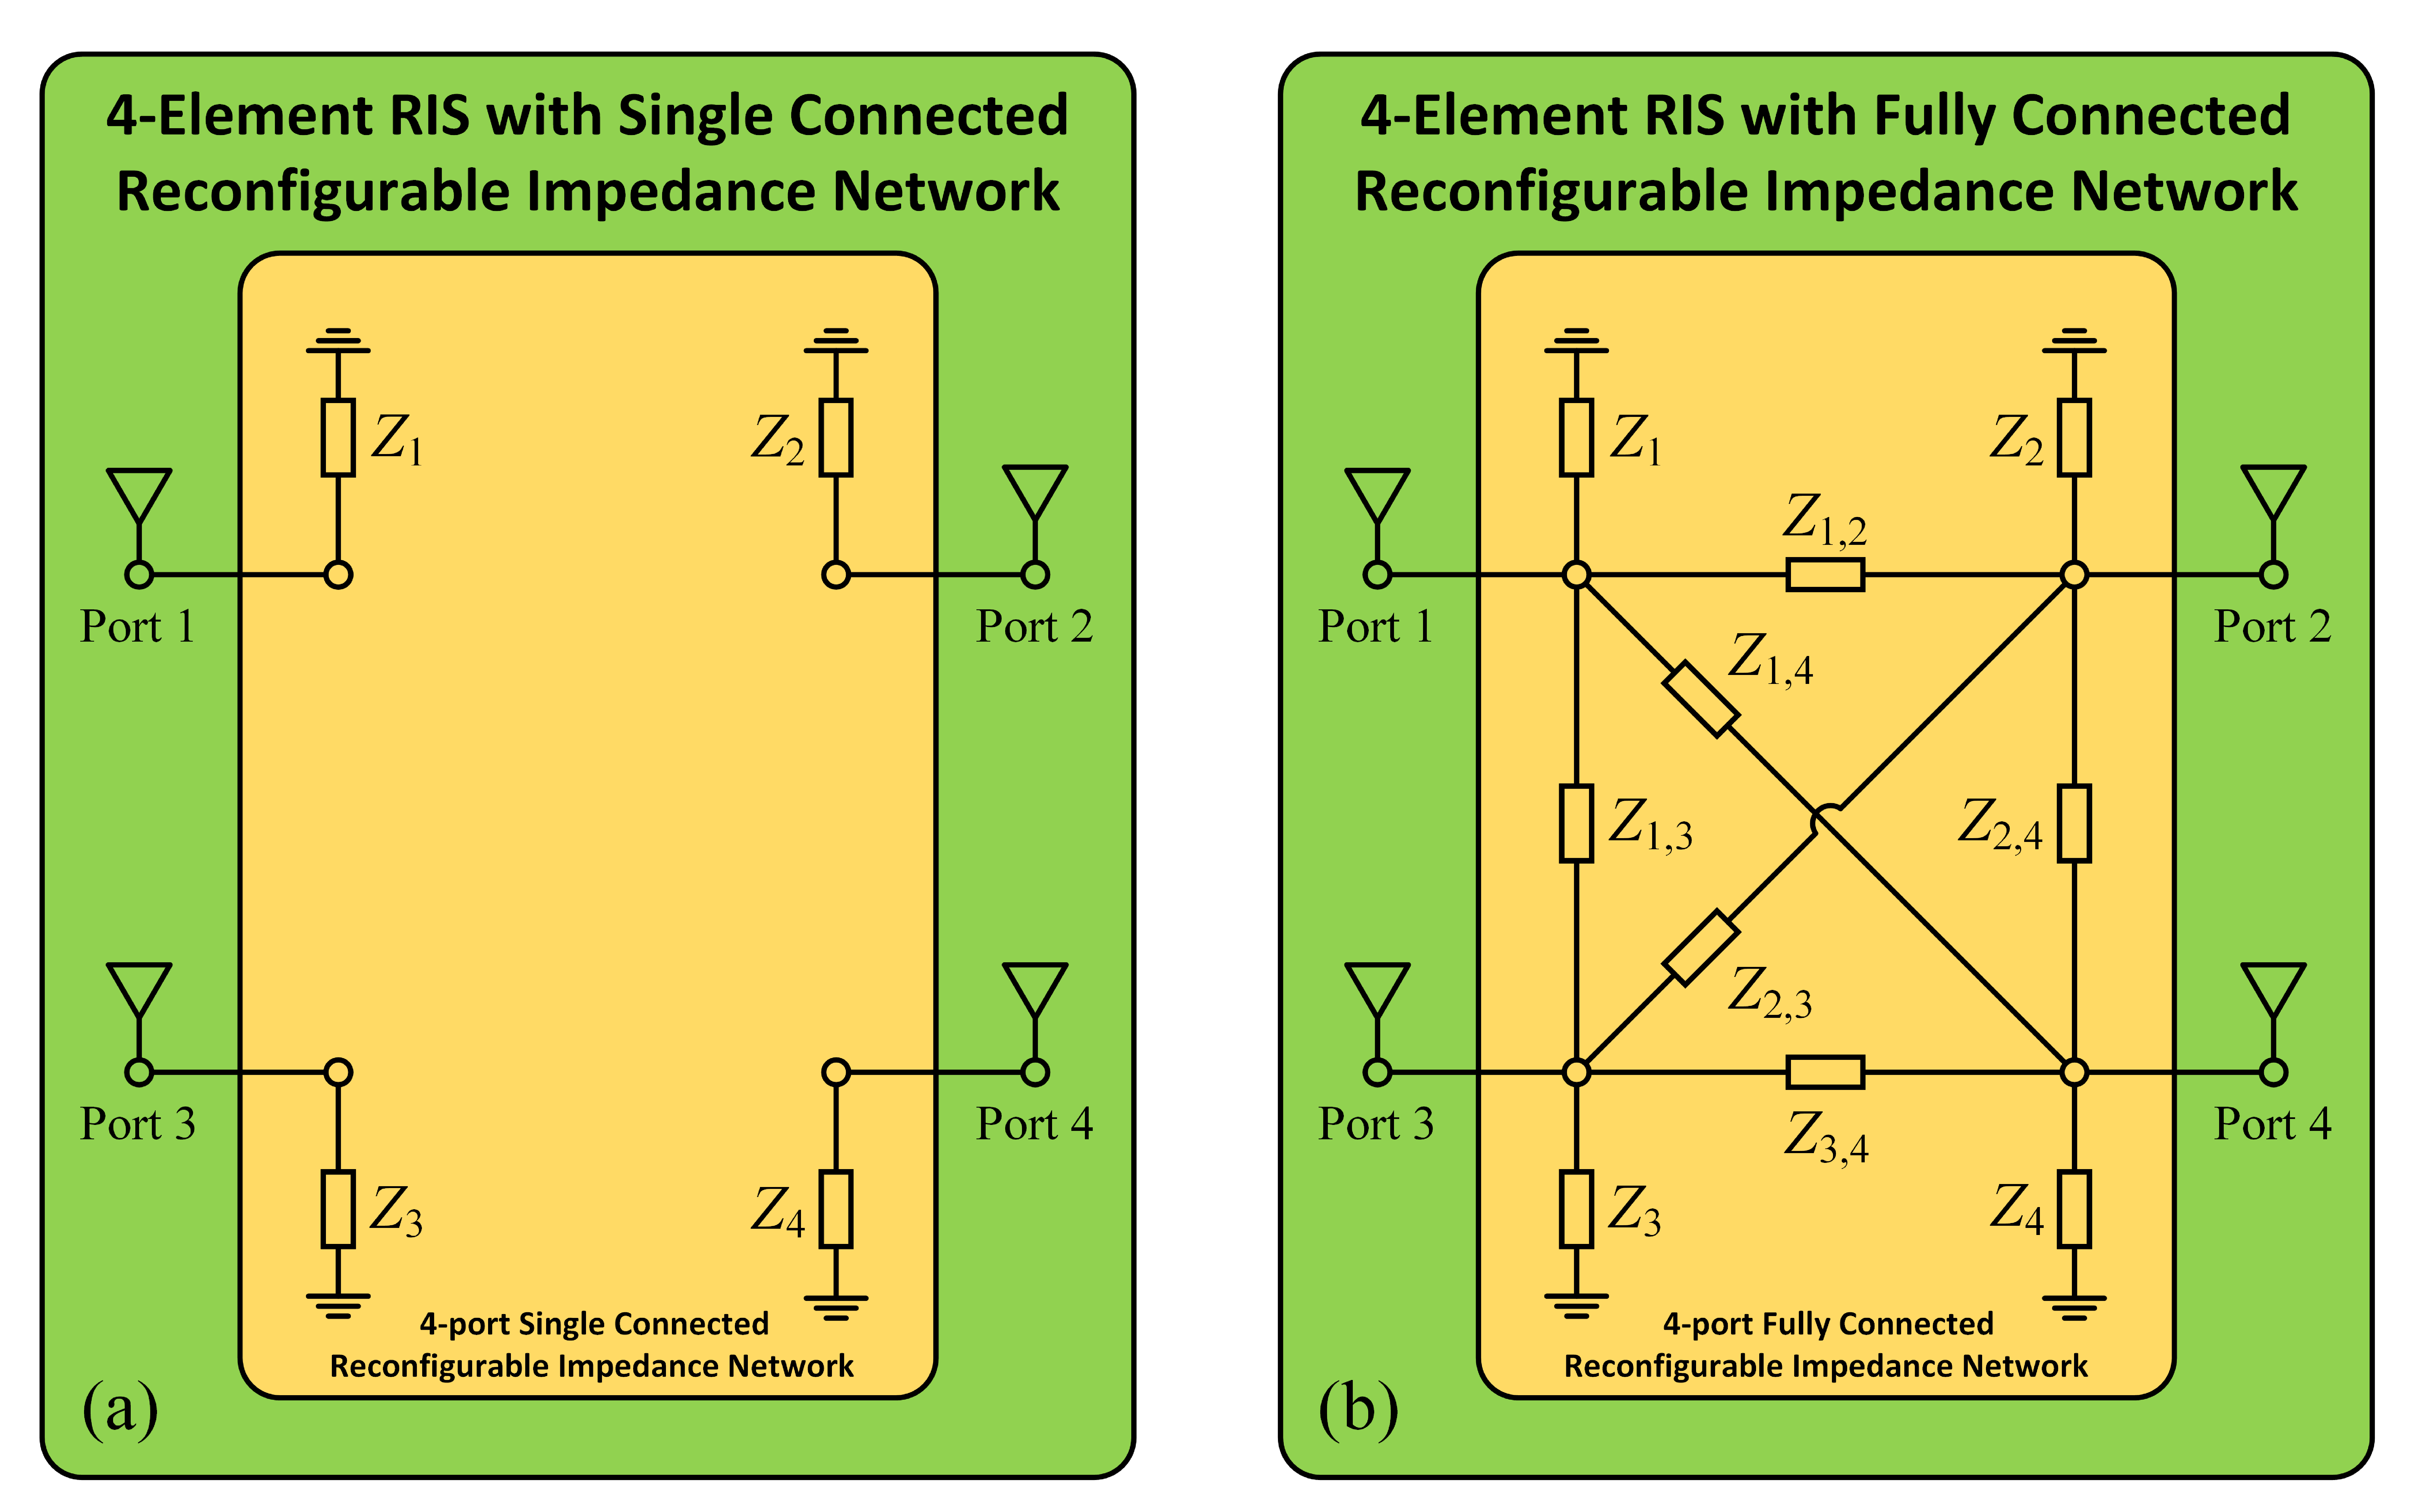
\includegraphics{../assets/viva/bd_ris_architecture_1.eps}
				}
				\caption{Architecture of diagonal and \gls{bd}-\gls{ris} \cite{Shen2020a}}
				\label{fg:bd_ris_architecture_2}
			\end{figure}

		\end{block}
	\end{frame}

	\begin{frame}{Proposed geodesic update via Lie algebra}
		\vspace{-0.25cm}
		\begin{figure}
			\centering
			\includegraphics[width=0.5\textwidth]{../assets/viva/lie_group.pdf}
		\end{figure}
		\vspace{-0.25cm}
		\begin{block}{Non-geodesic vs geodesic \gls{rcg}}
			\begin{itemize}
				\item Non-geodesic: add then retract
				\begin{equation*}
					\bar{\mathbf{\Theta}}_g^{(r+1)} = \mathbf{\Theta}_g^{(r)} + \mu \mathbf{D}_g^{(r)}, \quad \mathbf{\Theta}_g^{(r+1)} = \bar{\mathbf{\Theta}}_g^{(r+1)} \bigl({\bar{\mathbf{\Theta}}_g^{(r+1)\mathsf{H}}} \bar{\mathbf{\Theta}}_g^{(r+1)}\bigr)^{-1/2}
				\end{equation*}
				\item Geodesic: multiplicative and rotational update
				\begin{equation*}
					\mathbf{\Theta}_g^{(r+1)} = \mathbf{G}_g^{(r)}(\mu) = \exp(\mu \mathbf{D}_g^{(r)}) \mathbf{\Theta}_g^{(r)}
					\label{eq:update_geodesic}
				\end{equation*}
			\end{itemize}
		\end{block}
		\begin{exampleblock}{Performance comparison}
			\begin{table}
				\label{tb:complexity_test}
				\centering
				\tiny
				\begin{tabular}{ccccccc}
					\toprule
					\multirow{2}{*}{\gls{rcg} path} & \multicolumn{3}{c}{$N_\mathrm{S}=16$} & \multicolumn{3}{c}{$N_\mathrm{S}=256$}                                                               \\ \cmidrule(lr){2-4} \cmidrule(lr){5-7}
													& Objective                             & Iterations                             & Time [s]         & Objective        & Iterations & Time [s] \\ \midrule
					Geodesic                        & $\num{4.359e-3}$                      & 11.59                                  & $\num{1.839e-2}$ & $\num{1.163e-2}$ & 25.58      & 3.461    \\
					Non-geodesic                    & $\num{4.329e-3}$                      & 30.92                                  & $\num{5.743e-2}$ & $\num{1.116e-2}$ & 61.40      & 13.50    \\ \bottomrule
				\end{tabular}
			\end{table}
		\end{exampleblock}
	\end{frame}

	\begin{frame}{Problem formulation}
		\begin{block}{Pareto frontier of channel singular values}
			\vspace{-0.25cm}
			\begin{maxi*}
				{\scriptstyle{\mathbf{\Theta}}}{\sum_n \rho_n \sigma_n(\mathbf{H})}{}{}
				\addConstraint{\mathbf{\Theta}_g^\mathsf{H} \mathbf{\Theta}_g=\mathbf{I},}{\quad \forall g,}{}
			\end{maxi*}
		\end{block}
		\begin{block}{Achievable rate maximization}
			\vspace{-0.25cm}
			\begin{maxi*}
				{\scriptstyle{\mathbf{W},\mathbf{\Theta}}}{R = \log \det \biggl(\mathbf{I} + \frac{\mathbf{W}^\mathsf{H}\mathbf{H}^\mathsf{H}\mathbf{H}\mathbf{W}}{\eta}\biggr)}{}{}
				\addConstraint{\lVert \mathbf{W} \rVert _\mathrm{F}^2}{\le P}
				\addConstraint{\mathbf{\Theta}_g^\mathsf{H} \mathbf{\Theta}_g}{=\mathbf{I}, \quad \forall g.}
			\end{maxi*}
		\end{block}
		\begin{exampleblock}{Solution by group-wise geodesic \glsfmtshort{rcg}}
			\begin{itemize}
				\item Faster convergence thanks to appropriate parameter space
				\item Optimal and low-complexity solutions
			\end{itemize}
		\end{exampleblock}
	\end{frame}

	\begin{frame}{Simulation results: Singular value and achievable rate}
		\begin{figure}
			\centering \hspace*{-1cm}
			\subfloat[$2 \times 32 \times 2$\label{fg:singular_pareto_sx32}]{
				\resizebox{!}{3.2cm}{
					\input{../assets/viva/singular_pareto_sx32.tex}
				}
			}
			\subfloat[$4 \times 32 \times 4$ (rank-1)\label{fg:singular_bound_rank2_sx128}]{
				\resizebox{!}{3.2cm}{
					\input{../assets/viva/singular_bound_rank2_sx128.tex}
				}
			}
			\subfloat[$N_\mathrm{T} \times 128 \times N_\mathrm{R}$\label{fg:rate_txrx}]{
				\resizebox{!}{3.1cm}{
					\input{../assets/viva/rate_txrx.tex}
				}
			}
		\end{figure}
		\vspace{1em}
		\begin{itemize}
			\item \gls{bd}-\gls{ris} provides \qty{22}{\percent} and \qty{38}{\percent} dynamic range gain for $\sigma_1(\mathbf{H})$ and $\sigma_2(\mathbf{H})$
			\item Asymptotic bounds are valid for diagonal and \gls{bd}-\gls{ris}
			\item Percentage rate gain of \gls{bd}-\gls{ris} scales with \gls{mimo} dimension and group size
		\end{itemize}
	\end{frame}
\end{section}

\bibliographystyle{IEEEtran}
\bibliography{../misc/library.bib}
\end{document}
